\hypertarget{section-runtime-view}{%
\section{Runtime View}\label{section-runtime-view}}

\hypertarget{__runtime_scenario_1}{%
\subsection{Display Product List}\label{__runtime_scenario_1}}
\begin{figure}[h]
  \centering
  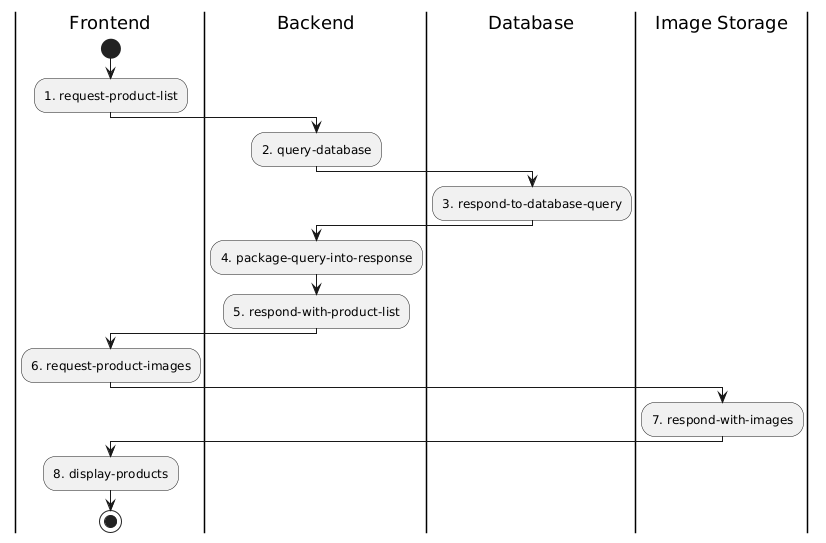
\includegraphics[width=\textwidth]{images/uml_swimlane_product_list.png}
  \caption{UML Swimlane Diagram for Displaying Product List}
\end{figure}

Explanation:
\begin{enumerate}
  \item Frontend request product list from backend.
  \item The backend queries the database to retrieve all the products.
  \item The database responds to the query with the products.
  \item The backend packages the result of the query into a JSON response.
  \item The backend sends the response to the frontend.
  \item Since the backend response contains URLs to images rather than the images themselves, the frontend needs to fetch it from the BLOB Storage.
  \item Read operations can be carried out anonymously on the images, therefore the BLOB storage responds with the image data.
  \item Now the product list can be displayed in the frontend.
\end{enumerate}

\newpage
\hypertarget{__runtime_scenario_2}{%
\subsection{Cart Checkout Process}\label{__runtime_scenario_2}}
\begin{figure}[!h!]
  \centering
  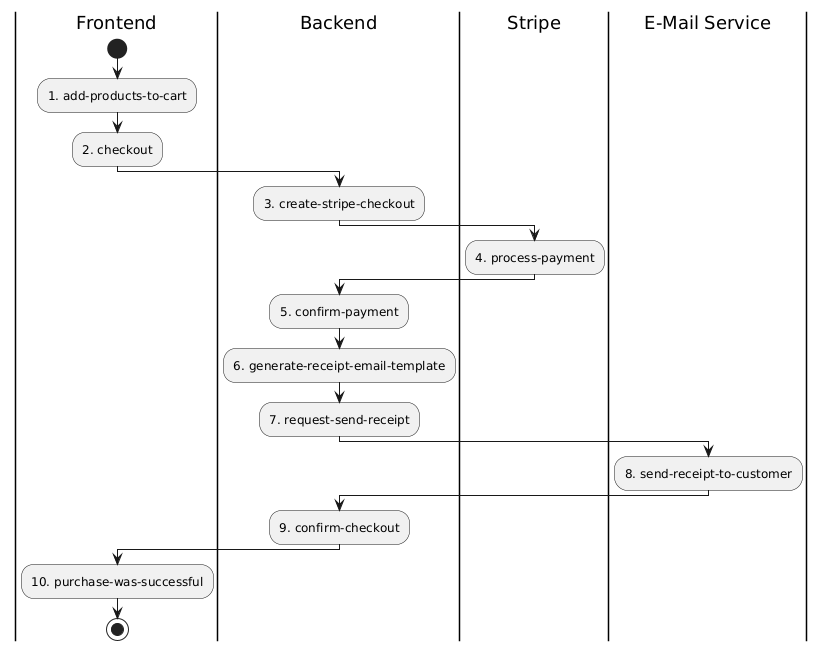
\includegraphics[width=0.9\textwidth]{images/uml_swimlane_checkout.png}
  \caption{UML Swimlane Diagram for the Checkout Process}
\end{figure}

Explanation:
\begin{enumerate}
  \item The user uses the frontend user interface to add items to the cart.
  \item The user wants to start the checkout process.
  \item The backend creates a checkout on the Stripe platform.
  \item The Stripe platform handles the payment process such as accepting credit card information.
  \item The backend confirms whether the payment with Stripe was successful.
  \item The backend generates a template E-Mail containing an order confirmation with a receipt as a PDF attachment.
  \item The backend forwards this E-Mail to the E-Mail Service, so that it can be sent to the user.
  \item The E-Mail Service sends the order confirmation and receipt to the user's E-Mail address.
  \item The backend confirms that the checkout was successful.
  \item The transaction is shown as successful in the frontend user interface.
\end{enumerate}

\hypertarget{__runtime_scenario_3}{%
\subsection{Creating/Updating/Deleting Products in Admin Panel}\label{__runtime_scenario_3}}
\begin{figure}[h]
  \centering
  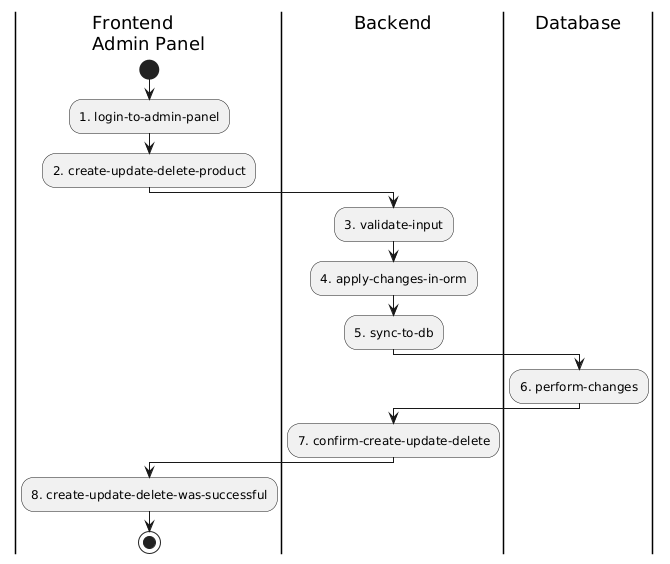
\includegraphics[width=\textwidth]{images/uml_swimlane_product_create_update_delete.png}
  \caption{UML Swimlane Diagram for Creating, Updating, and Deleting Products via the Admin Panel}
\end{figure}

Explanation:
\begin{enumerate}
  \item An administrator logs into the admin panel with admin credentials.
  \item The administrator creates, updates and/or deletes product(s).
  \item The backend performs input validation to e.g., prevent negative prices or invalid input formats.
  \item The operation is carried out using the object relational mapping of the backend.
  \item The object relational mapping syncs up with the database.
  \item The database performs the required write operations.
  \item The backend confirms, that the operation was successful.
  \item The administrator now receives feedback, that the operation was successful.
\end{enumerate}
